The Android application used to control the Mecanum wheel car was developed in Kotlin and built using Android Studio. The primary motivation behind creating the app was to offer a smartphone-based control system for the car via WiFi, using UDP packets for communication. This system offers a simple interface for directional movement, speed control, and vehicle status feedback, all integrated into an intuitive layout designed for ease of use, which can be seen in fig.~\ref{fig:AppScreenshot}.

\begin{figure}[h]
	\centering
	\captionsetup{justification=centering}
	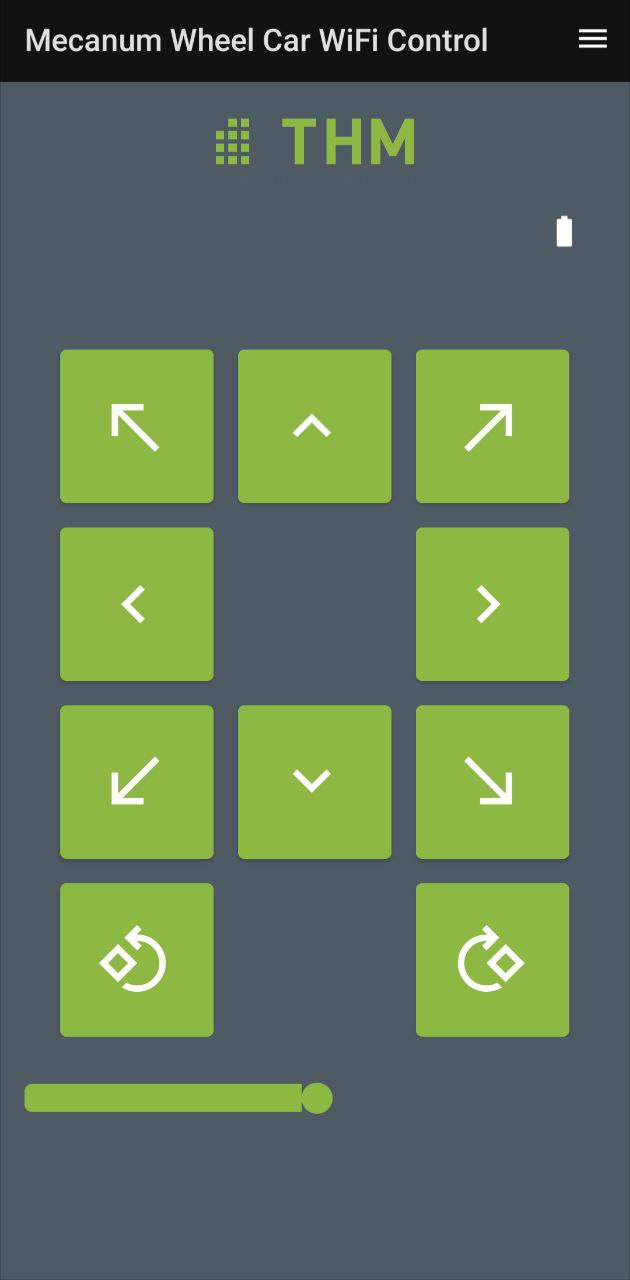
\includegraphics[width=0.3\linewidth]{App_Screenshot.jpg}
	\caption{Screenshot from the Android App}
	\label{fig:AppScreenshot}
\end{figure}

The app allows users to control the car by sending directional commands to move the car in one of eight base directions—up, down, left, right, and the diagonals—using on-screen buttons. Additionally, users can rotate the car clockwise or counterclockwise using designated buttons. The interface ensures that each directional button initiates movement when pressed and sends a "stop" command as soon as the button is released. If a button is pressed for longer than 8 seconds, the app sends a "keepalive" message, ensuring the car does not time out due to inactivity.
At the bottom of the screen, a slider allows the user to adjust the speed of the car dynamically, ranging from slow to fast movement. The speed value is converted into control commands that are transmitted via UDP to the car.\\
The layout of the app consists of three key areas:
\begin{itemize}
	\item \textbf{Directional Buttons}: These are located centrally on the screen and allow users to control the car's movement. Each button corresponds to one of the eight base directions or rotation commands (clockwise and counterclockwise).
	\item \textbf{Speed Control Slider}: Positioned at the bottom, this slider allows users to adjust the car's speed. The value is continuously read and used to form the movement command strings sent over UDP.
	\item \textbf{Status Area}: The top of the app displays a battery symbol, which is updated with real-time information about the car’s battery status and motor activity, based on UDP status messages sent by the car.
\end{itemize}

To control the car, the app transmits UDP packets to the Mecanum car, which is set to the IP address "192.168.10.1" on port 4444. A mapping function inside the app converts button presses into the respective command strings in the format "rc x y z". Here, x and y represent the speed in the respective direction, and z indicates rotation speed. The app ensures that each command reflects the user's intended movement, and every release of a button triggers a "stop" command to halt the car.
The app makes use of the keepalive-mechanism, which is automatically triggered if a button is held down for more than 8 seconds. The app sends this message to prevent the car from entering a timeout state during continuous use. The keepalive packet is sent periodically to maintain the connection and avoid interruptions in operation.\\
In addition to sending movement commands, the app listens for status updates from the car on UDP port 4445. These updates contain vital information about the car’s battery voltage and motor performance, which are displayed in the status area at the top of the screen. The data is presented clearly for the user, with battery voltage and percentage shown next to a battery icon, while individual motor performance is displayed in terms of percentage. The app’s interface also includes a battery status checker, which updates in real time based on incoming messages from the car. This ensures that the user can monitor the car’s battery condition and make informed decisions about operational time.\\
Though the current version of the app provides a reliable interface for controlling the Mecanum car, future iterations could integrate additional features such as customizable control schemes or enhanced feedback, such as warnings when the battery is low.
This Kotlin-based application forms a robust foundation for further development, ensuring that users can control the car seamlessly over WiFi, with real-time status monitoring and intuitive controls.